\documentclass[ignorenonframetext,]{beamer}
\setbeamertemplate{caption}[numbered]
\setbeamertemplate{caption label separator}{: }
\setbeamercolor{caption name}{fg=normal text.fg}
\beamertemplatenavigationsymbolsempty
\usepackage{color}
\usepackage{lmodern}
\usepackage{inconsolata}
\usepackage{amssymb,amsmath}
\usepackage{ifxetex,ifluatex}
\usepackage{adjustbox} % adjust text size to fit slide
\usepackage{fixltx2e} % provides \textsubscript
\ifnum 0\ifxetex 1\fi\ifluatex 1\fi=0 % if pdftex
  \usepackage[T1]{fontenc}
  \usepackage[utf8]{inputenc}
\else % if luatex or xelatex
  \ifxetex
    \usepackage{mathspec}
    \usepackage{fontspec}
  \else
    \usepackage{fontspec}
  \fi
  \defaultfontfeatures{Ligatures=TeX,Scale=MatchLowercase}
\fi
% use upquote if available, for straight quotes in verbatim environments
\IfFileExists{upquote.sty}{\usepackage{upquote}}{}
% use microtype if available
\IfFileExists{microtype.sty}{%
\usepackage{microtype}
\UseMicrotypeSet[protrusion]{basicmath} % disable protrusion for tt fonts
}{}
\newif\ifbibliography
\usepackage{longtable,booktabs}
\usepackage{caption}
% These lines are needed to make table captions work with longtable:
\makeatletter
\def\fnum@table{\tablename~\thetable}
\makeatother

% Prevent slide breaks in the middle of a paragraph:
\widowpenalties 1 10000
\raggedbottom

\AtBeginPart{
  \let\insertpartnumber\relax
  \let\partname\relax
  \frame{\partpage}
}
\AtBeginSection{
  \ifbibliography
  \else
    \let\insertsectionnumber\relax
    \let\sectionname\relax
    \frame{\sectionpage}
  \fi
}
\AtBeginSubsection{
  \let\insertsubsectionnumber\relax
  \let\subsectionname\relax
  \frame{\subsectionpage}
}

\setlength{\emergencystretch}{3em}  % prevent overfull lines
\providecommand{\tightlist}{%
  \setlength{\itemsep}{0pt}\setlength{\parskip}{0pt}}
\setcounter{secnumdepth}{0}
%gets rid of bottom navigation bars
\setbeamertemplate{footline}[frame number]{}

%gets rid of bottom navigation symbols
\setbeamertemplate{navigation symbols}{}

%gets rid of footer
%will override 'frame number' instruction above
%comment out to revert to previous/default definitions
%\setbeamertemplate{footline}{}

%%%%%%%%%%%%%%%%%%%%%%%%%%%%%%%%%%%%%%%%%%%%%%%%%%%%%%%%%%%%%%%%%%%%%%%%%%%%%%%
% Title slide
%%%%%%%%%%%%%%%%%%%%%%%%%%%%%%%%%%%%%%%%%%%%%%%%%%%%%%%%%%%%%%%%%%%%%%%%%%%%%%%

\title{\Large
En förhandstitt på verktyget för \\ normalisering av andraspråkstexter
}

\author{\large Dan Rosén \\
}

\date{\large Språkbankens höstworkshop 2017
  \vspace{1cm}
  \\
  
\includegraphics[height=1.6cm]{logo_gu.png}
  \hspace{5cm}
  
\includegraphics[height=1.4cm]{logo_sb.jpg}
}


\begin{document}
\frame{\titlepage}

%%%%%%%%%%%%%%%%%%%%%%%%%%%%%%%%%%%%%%%%%%%%%%%%%%%%%%%%%%%%%%%%%%%%%%%%%%%%%%%
% Slides
%%%%%%%%%%%%%%%%%%%%%%%%%%%%%%%%%%%%%%%%%%%%%%%%%%%%%%%%%%%%%%%%%%%%%%%%%%%%%%%

\begin{frame}
\frametitle{SweLL:
Forskningsinfrastruktur för svenska som andraspråk}
\begin{itemize}
\item GU: Elena Volodina, Julia Prentice, Monica Reichenberg
\item SU: Mats Wirén, Gunlög Sundberg
\item UU: Beata Megyesi
\item UmU: Lena Granstedt
\item Riksbankens Jubileumsfond under 2017-2019
\vspace{\baselineskip}
\item insamling av $\geq$600 inlärartexter
\item normalisera: transformera texten m.a.p. ``normspråket''
\item annotera efter en avvikelsetaxonomi
\end{itemize}
\end{frame}

\begin{frame}
\frametitle{Exempel på inlärartext och normalisering}

\includegraphics[width=\textwidth, trim={0 3.3cm 0 0}, clip]{ladder_black.pdf}
\pause
\vspace{0.66cm}


\includegraphics[width=\textwidth, trim={0 0 0 3.3cm}, clip]{ladder_black.pdf}
\end{frame}

\begin{frame}
\frametitle{Exempel som parallellkorpus}

\includegraphics[width=\textwidth]{ladder_black.pdf}
\end{frame}

\begin{frame}
\frametitle{Exempel som annoterad parallellkorpus}
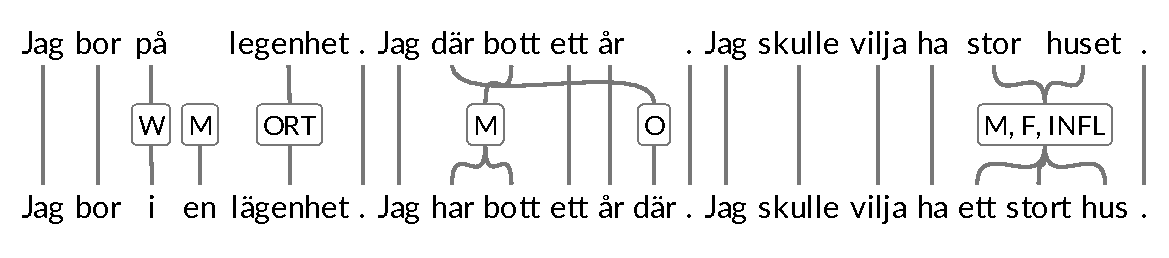
\includegraphics[width=\textwidth]{labelled_ladder_black.pdf}
\end{frame}

\begin{frame}[fragile]
\frametitle{Demo}
\begin{center}
%\large
\url{http://demo.spraakdata.gu.se/dan/swell-editor}
\end{center}
\end{frame}

\begin{frame}
\frametitle{Sammanfattning}
\begin{itemize}
\item Verktyg för normalisering och annotering av inlärartexter
\item Separation mellan dessa två aktiviteter
\item Skapar parallellt en parallellkorpus
\end{itemize}
\vspace{1cm}
Nästa steg:
\begin{itemize}
\item Utveckling av avvikelsetaxonomin
\item Internt pilotannoteringsprojekt
\end{itemize}
\vspace{1cm}
\url{http://demo.spraakdata.gu.se/dan/swell-editor}
\end{frame}

\end{document}
